\chapter{CellTAN Application} \label{chap:chap5}


\section{Case study}


The experiments validating CellTAN's behavior incorporate two neighboring grid-tied string inverters from the same PV farm with common satellite data. Their only known characteristics are:

\begin{itemize}
    \item Inverter one: 12.5kW nominal power; 14.4kW peak power; fixed tilt and azimuth; installed January 1st, 2013.
    \item Inverter two: 15kW nominal power; 15.84kW peak power; fixed tilt and azimuth; installed January 1st, 2013.
\end{itemize}

\begin{table}[h!]
\caption{Available variables from two inverters and a satellite.}
\label{tab:availablevariables}
\resizebox{\textwidth}{!}{%
\begin{tabular}{|l|l|l|l|}
\hline
\multicolumn{1}{|c|}{\textbf{Variable}} & \multicolumn{1}{c|}{\textbf{Source}} & \multicolumn{1}{c|}{\textbf{Unit}} & \multicolumn{1}{c|}{\textbf{Label}} \\ \hline
AC side power                           & Inverter (1 \& 2)                    & W                                  & ac\_power                           \\ \hline
AC side current                         & Inverter (1 \& 2)                    & A                                  & ac\_current                         \\ \hline
AC side voltage                         & Inverter (1 \& 2)                    & V                                  & ac\_voltage                         \\ \hline
DC side power                           & Inverter (1 \& 2)                    & W                                  & dc\_power                           \\ \hline
DC side current                         & Inverter (1 \& 2)                    & A                                  & dc\_current                         \\ \hline
DC side voltage                         & Inverter (1 \& 2)                    & V                                  & dc\_voltage                         \\ \hline
Global tilted irradiance                & Satellite                            & W/m\textsuperscript{2}             & global\_tilted\_irradiance          \\ \hline
Global horizontal irradiance            & Satellite                            & W/m\textsuperscript{2}             & global\_horizontal\_irradiance      \\ \hline
Cloud coverage                          & Satellite                            & \%                                 & cloud\_coverage                     \\ \hline
Air temperature                         & Satellite                            & ºC                                 & temperature                         \\ \hline
\end{tabular}%
}
\end{table}

Table \ref{tab:availablevariables} represents the available variables and corresponding labels used to identify them in the cell's inputs and graphs. These variables are sampled every 10 minutes from May 31, 2020, at 5:00 am to April 30, 2023, at 7:30 pm (with gaps). We utilized data from 2020 until the end of 2022 for the cells' knowledge base, and any information from 2023 onwards is considered new and used for testing. Since there is no production at night, the data's original database does not store values for this period. Not accounting for the night as missing samples, we have around 98\% of data availability.

Analyzing and cleaning raw inverter and satellite data is essential to take full benefit of CellTAN's capabilities. As seen in its formulation stage, having a clean knowledge base contributes to correctly identifying anomalous situations. Therefore, the following sections focus on these two steps, contributing to understanding the anomalies' domain and frequency of occurrence.

\subsection{Data analysis}

Before data visualization, and regarding the variables in table \ref{tab:availablevariables}, we eliminate those that will not benefit the CellTAN. We determined that AC side voltage is insignificant since the grid mandates it in a grid-tied inverter. We have decided to only use the measure of power instead of using the AC side current measure since, in conjunction with voltage, it provides the same information. To simplify things further, we do not need to consider the power on the DC if considering both the DC side current and voltage measures.

We examine all variables related to satellite data to determine which ones could be useful, not making any premature assumptions.

\subsubsection{Power}


\begin{figure}[h!]
    \centering
    \includegraphics[width=\textwidth]{figures/chapter5/analysis/00_power_kb.pdf}
    \caption{Inverter AC side power from 2020 to 2022, used for the knowledge base.}
    \label{fig:eda_power_kb}
\end{figure}

Figure \ref{fig:eda_power_kb} shows the power profile of the two studied inverters. Right away, we notice that the power of inverter two caps at around 14kW, while inverter one usually maxes at 12kW. This information is coherent with their ratings. We can notice two relatively large chunks of missing data, with the gaps occurring in mid to late 2022.

\begin{figure}[h!]
    \centering
    \includegraphics[width=\textwidth]{figures/chapter5/analysis/01_power_test.pdf}
    \caption{Inverter AC side power from 2023-01-01 to 2023-01-05, used for testing.}
    \label{fig:eda_power_test}
\end{figure}

Figure \ref{fig:eda_power_test} represents the power profile on the portion of data used for testing. When performing a closer inspection (with more zoom), we could hand-pick some fault occurrences in both datasets, with the majority being one inverter off while the other continues regular operation. However, these will be more noticeable during different types of data analysis, such as pair plotting. Regardless, the cases that will matter are in the test data since these scenarios will not exist in the knowledge after cleaning. In Section \ref{subsec:results}, you will find a selection of carefully chosen scenarios.

\begin{figure}[h!]
    \centering
    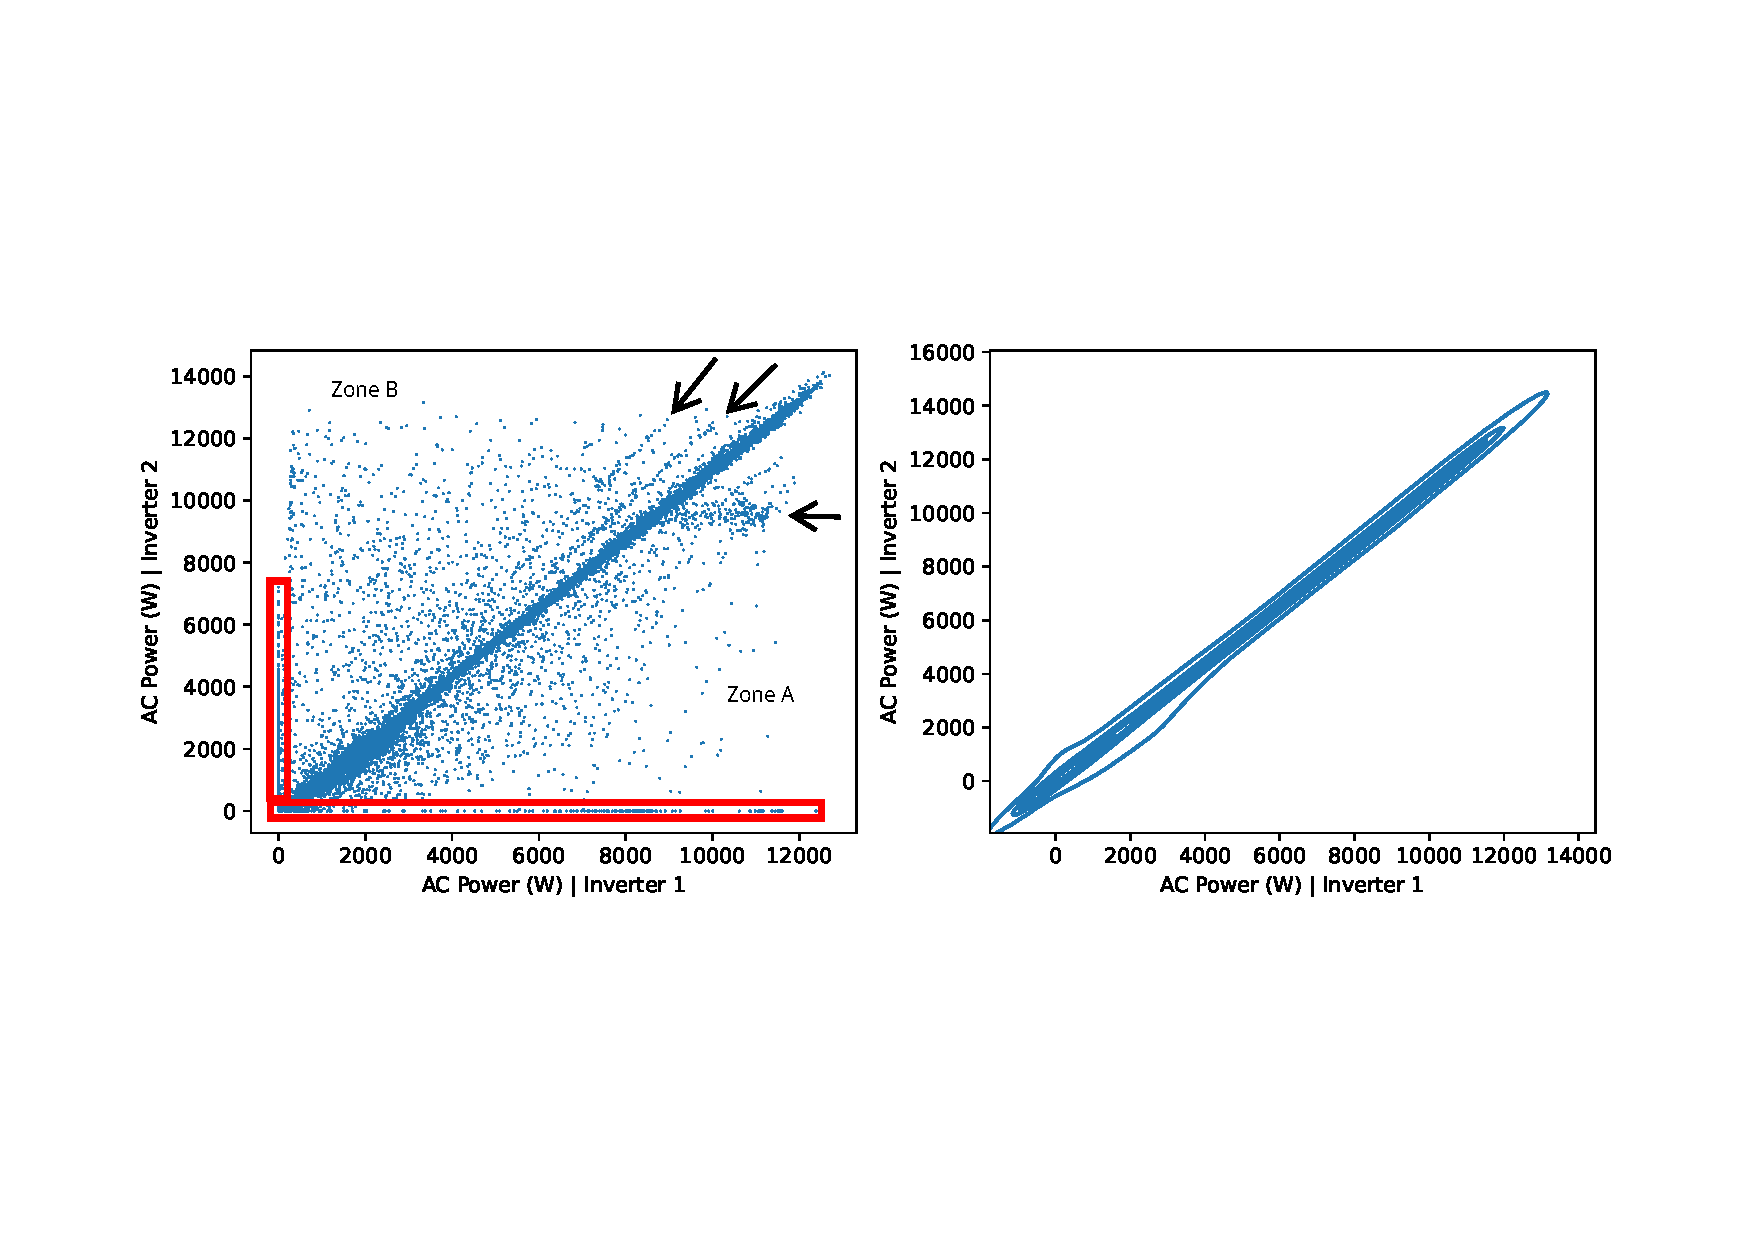
\includegraphics[width=\textwidth,trim={0 5.5cm 0cm 5.5cm},clip]{figures/chapter5/analysis/02_power_pairplots_kb_annotated.pdf}
    \caption{Pair plot of AC power from both inverters (2020 to 2022), using scatter (left) and KDE (Kernel Density Estimation) (right).}
    \label{fig:eda_power_kb_pair}
\end{figure}

Figure \ref{fig:eda_power_kb_pair} lets us better understand the relationship between the two inverters. As expected, since they are neighboring, they have a strong trend line, leading them to a high Pearson coefficient: 0.97753. However, the noise from outliers is noticeable in the scatter. We define Zone A as the zone where inverter two underperforms compared to one and Zone B as the opposite. The black arrows in the graph display secondary trend lines in Zone B, indicating scenarios of inverter one performing consistently less than expected. Another arrow also points out a cloud in Zone A (right under the trend line) of the opposite scenario. Furthermore, the red rectangles highlight instances where one inverter was functioning while the other was not. CellTAN must flag these situations, so we should remove them from the knowledge base.
The KDE visualization confirms that most samples lie close to the primary trend.

\begin{figure}[h!]
    \centering
    \includegraphics[width=\textwidth]{figures/chapter5/analysis/03_power_pairplots_test.pdf}
    \caption{Pair plot of AC power from both inverters (2023), using scatter (left) and KDE (Kernel Density Estimation) (right).}
    \label{fig:eda_power_test_pair}
\end{figure}

From \ref{fig:eda_power_test_pair}, it is clear that test data has fewer outliers than the previous. Nonetheless, there are many occurrences of inverter one being inoperational. Besides, there are also a considerable amount of samples below the trend line, meaning the underperformance of inverter two.

% dizer que tem menos outliers, mas várias situações com o inversor 1 inoperacional

\subsubsection{Voltage and Current} \label{subsubsec:eda_volt_curr}

Both inverters are equipped with MPPTs to maximize the power output from their strings. As a result of this power converter, the current and voltage readings should fall within the optimal range of the I-V curve.

\begin{figure}[h!]
    \centering
    \includegraphics[width=\textwidth,trim={0 5.5cm 0cm 5.5cm},clip]{figures/chapter5/analysis/04_voltage_current_pairplot_kb_1_annotated.pdf}
    \caption{Pair plot of DC side voltage and current from inverter one (2020-2022), using scatter (left) and KDE (Kernel Density Estimation) (right).}
    \label{fig:eda_volt_curr_pair_kb_1}
\end{figure}

\begin{figure}[h!]
    \centering
    \includegraphics[width=\textwidth,trim={0 5.5cm 0cm 5.5cm},clip]{figures/chapter5/analysis/06_voltage_current_pairplot_kb_2_annotated.pdf}
    \caption{Pair plot of DC side voltage and current from inverter two (2020-2022), using scatter (left) and KDE (Kernel Density Estimation) (right).}
    \label{fig:eda_volt_curr_pair_kb_2}
\end{figure}

Regarding DC side voltage and current, figures \ref{fig:eda_volt_curr_pair_kb_1} and \ref{fig:eda_volt_curr_pair_kb_2} demonstrate the operating range of the inverter's MPPT. Both kickstart production at around 400 V and operate until close to 600 V. Between this range, the central column of samples represents voltage-current points relative to the knee of the strings' I-V curve (see figure \ref{fig:mpptcurve}), with irradiance generally increasing along its height. Some instances are outside this normal operation range (outliers), especially in the zone marked by the black arrow. This zone has particular interest given that it represents scenarios of underperformance, which could mean the occurrence of faults. It is denser in figure \ref{fig:eda_volt_curr_pair_kb_2}, meaning that inverter two has more underperforming situations, which was not completely clear from the previous analysis (figure \ref{fig:eda_power_kb_pair}). Appendix \ref{ap2:eda} presents the same charts, but for test data (figures \ref{fig:eda_voltage_current_test_1} and \ref{fig:eda_voltage_current_test_2}).

\subsubsection{Satellite} \label{subsubsec:eda_sat}

Irradiance should be the satellite variable most related to inverters' power. Therefore, we scatter both tilted and horizontal irradiance against AC power from inverters one and two.

\begin{figure}[h!]
    \centering
    \includegraphics[width=0.8\textwidth]{figures/chapter5/analysis/08_power_irrad_pairplot_scatter_kb.pdf}
    \caption{Scatter pair plot of the AC power, tilted and horizontal global irradiance for both inverters (2020 to 2022).}
    \label{fig:eda_power_irrad_pair_kb}
\end{figure}

Figure \ref{fig:eda_power_irrad_pair_kb} shows the relationship between irradiance and AC power. We expected a positive correlation, and it exhibits such. However, the large radius around the central trend line demonstrates cycles around it that resemble some kind of hysteresis (especially with horizontal irradiance). By adding a color that displays the hour in each sample, we can affirm that these paths occur due to the fixed nature of the installed PV panels, having a characteristic curve from low to high irradiance in the sunrise and another from high to low during the sunset. Because they produce more with less sunlight in the morning, we can infer that they are oriented slightly towards the east.

Although most instances appear inside the sunrise-sunset paths, there are some outliers. The most notable are the ones of non-zero irradiance with zero production. Either error in satellite data or some anomaly in the inverters causes these odd scenarios, so we target them for cleaning the knowledge base.

Regarding the rest of the meteorological variables (cloud coverage and temperature), we deemed them unnecessary since they do not demonstrate a direct relationship with inverter behavior (see figure \ref{fig:eda_irrelevant_meteo}). We added KDE visualizations and plots for the test period in appendix \ref{ap2:eda}.

% TODO colocar 09,10,11 nos anexos e mencionar

\subsection{Data Cleaning}

Now, we take our previous analysis and start the data-cleaning process. We used the Scikit-Learn Python Library and tried out some anomaly detection algorithms for outlier identification on our dataset: Robust Covariance \cite{Rousseeuw1999}, Isolation Forest \cite{Liu2008} \cite{Liu2012}, and Local Outlier Factor \cite{Breunig2000}. The code used for our plotting derived from an example made by Alexandre Gramfort, available on the Scikit-Learn website \cite{sklearn_example}.

\subsubsection{Power}

Based on the geographical proximity of the inverters, we have determined that the area around the trendline shown in figure \ref{fig:eda_power_kb} indicates standard operating points. Therefore, we must remove any samples deviating from this reference to clean the knowledge base.

\begin{figure}[h!]
    \centering
    \includegraphics[width=\textwidth]{figures/chapter5/cleaning/20_cleaning_power.pdf}
    \caption{Inliers (orange), outliers (blue), and decision boundaries (black) using three different anomaly detection algorithms on the AC Power from both inverters.}
    \label{fig:clean_power}
\end{figure}

In Figure \ref{fig:clean_power}, we can see a visual representation of various anomaly detection algorithms' inliers, outliers, decision boundaries, and their computation time (bottom right). These algorithms are fine-tuned for approximately 14\% of outlier contamination. Based on the results, we determined that the Robust Covariance algorithm was the most effective since it extracted the region around the trend line without issues. We selected it to clean our knowledge base.

\subsubsection{Satellite}

In section \ref{subsubsec:eda_sat}, we discovered that the inverters follow a standard production pattern based on the irradiance and hour of the day. The specific area within the paths is considered the central region of standard operation. To clean up the data, we will remove all other instances.

\begin{figure}[h!]
    \centering
    \includegraphics[width=\textwidth]{figures/chapter5/cleaning/21_cleaning_tilted_irrad.pdf}
    \caption{Inliers (orange), outliers (blue), and decision boundaries (black) using three different anomaly detection algorithms on the tilted irradiance and AC Power from both inverters.}
    \label{fig:clean_tilted_irrad}
\end{figure}

\begin{figure}[h!]
    \centering
    \includegraphics[width=\textwidth]{figures/chapter5/cleaning/22_cleaning_horizontal_irrad.pdf}
    \caption{Inliers (orange), outliers (blue), and decision boundaries (black) using three different anomaly detection algorithms on the horizontal irradiance and AC Power from both inverters.}
    \label{fig:clean_horizontal_irrad}
\end{figure}

Once again, figures \ref{fig:clean_tilted_irrad} and \ref{fig:clean_horizontal_irrad} demonstrate the effectiveness of the first algorithm, now for irradiance and power data. It is, once again, the chosen one for cleaning the knowledge base.

\subsubsection{Voltage and Current}

Cleaning voltage and current data were the most challenging thus far. The peculiar data distribution was an issue for all of the tested algorithms, and we combined them all to obtain the best inlier-outlier separation.

\begin{figure}[h!]
    \centering
    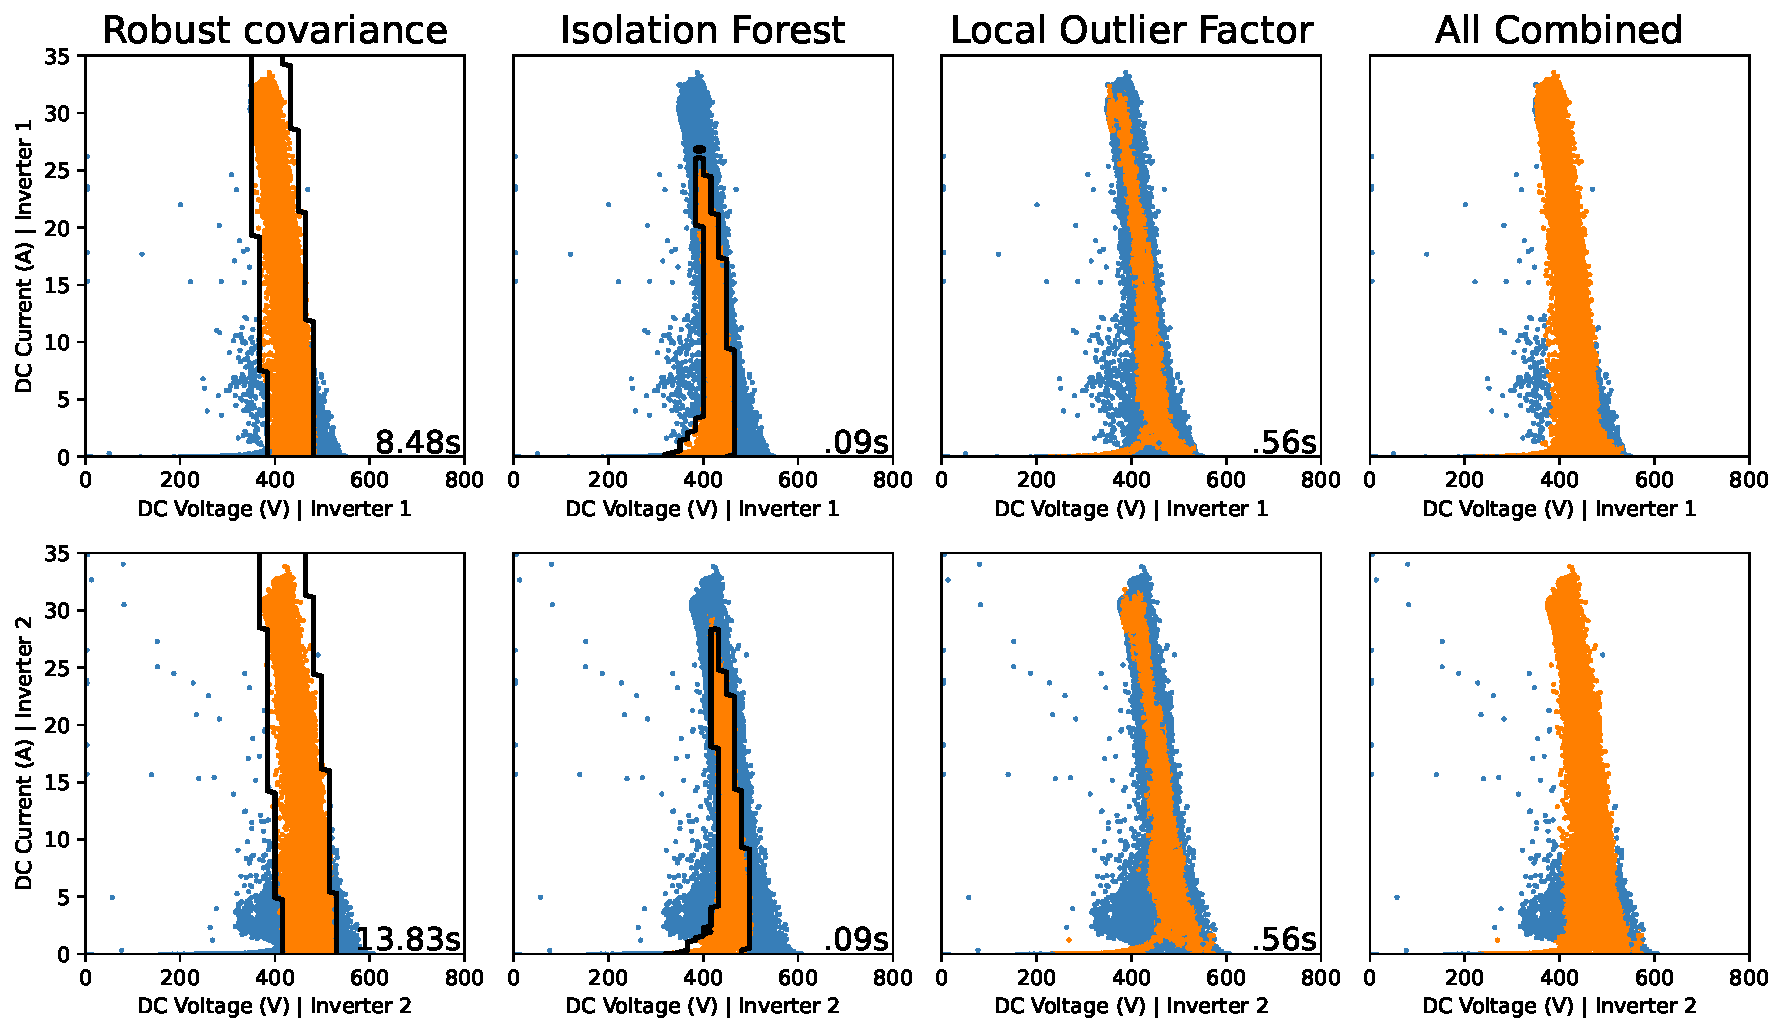
\includegraphics[width=\textwidth]{figures/chapter5/cleaning/23_cleaning_volt_curr.pdf}
    \caption{Inliers (orange), outliers (blue), and decision boundaries (black) using three different anomaly detection algorithms and their combination on the DC side voltage and current from both inverters.}
    \label{fig:clean_volt_curr}
\end{figure}

The charts in figure \ref{fig:clean_volt_curr} illustrates how the algorithms have difficulty keeping up with the data's distribution and preserving the densely populated areas. Neither algorithm effectively identifies the outliers separately, but their combination proved much more effective.

\subsection{Photovoltaic Plugin}

According to the CellTAN formulation, cells cannot share their variables' data directly to maintain privacy. As a result, this limits plugins to work with only the information available in the cell they are running in. Therefore, inverter underperformance is the only situation considered for the PV plugin, based on the analysis from section \ref{subsubsec:eda_volt_curr}. Access to both the inverter's data and satellite data allows the owner to employ other algorithms that leverage this knowledge for better situational and fault discernment, but this falls back to the "classical" centralized algorithms, which is not the scope of this work.



% flow chart de algoritmo para definição da fronteira de decisão
% fazer um diagrama super fixe com os passos do algoritmo ilustrados em desenho
To define the minimum operational boundary, we use the current and voltage samples resulting from the cleaning process to define inverter underperformance. Figure ref shows the proposed algorithm, which consists of the following steps:

\begin{itemize}
	\item Clean I-V data;
	\item Find the boundary points of lowest voltage;
	\item Fit a logarithmic function (\ref{eq:decayinglog}) to these points;
	\item Consider all points below the curve as situations of inverter underperformance.
\end{itemize}


Since data cleaning is already covered, we describe ways of determining the boundary points.
To begin, we establish bins for the current samples with a size of 1 A. Next, we examine each bin and determine the minimum voltage for that particular region via either the absolute minimum or a quantile. Once we have selected the reference minimum voltage, we record the bin's median current and minimum voltage as a boundary point.
After registering all boundary points, we use a curve-fitting algorithm to apply a decaying logarithmic function to them (equation \ref{eq:decayinglog}).

\begin{equation} \label{eq:decayinglog}
    V = a \times log(b \times I + c) + d \times I + e 
\end{equation}
where:
\begin{align*}
    V & : \text{Voltage (V)} \\
    I & : \text{Current (A)} \\
    a,b,c,d,e & : \text{Unknown curve parameters}
\end{align*}

\begin{figure}[h!]
    \centering
    \includegraphics[width=\textwidth]{figures/chapter5/algorithm/30_boundary.pdf}
    \caption{Inverter underperformance region based on the lowest boundary of current-voltage inliers.}
    \label{fig:anomaly_decision_boundary}
\end{figure}

Figure \ref{fig:anomaly_decision_boundary} illustrates the outcome of using the described algorithm on our case study inverters. With the fitted curve's parameters, the PV plugin can analyze a new sample and determine if it falls under the underperformance category—whenever it does, the plugin flags that situation and reports back to the cell.
The fitted logarithmic curves are:

$$
    V_{inverter1} = 19.2 \times log(170.7 \times I_{inverter1} - 37.0) - 2.5 \times I_{inverter1} + 269.5
$$

$$
    V_{inverter2} = 20.8 \times log(169.8 \times I_{inverter2} - 41.8) - 2.6 \times I_{inverter2} + 288.2 
$$

\subsection{CellTAN Configuration}

% config das células, como vai correr, como se simula o tempo
\dots

\subsection{Simulation and Results} \label{subsec:results}

\subsubsection{Inverter-Inverter mismatch}

\dots

\subsection{Inverters-Satellite mismatch}

\dots

\subsection{Inverter underperformance}

\dots

\subsection{Scaling up}

\dots

% \begin{figure}[h!]
%     \centering
%     \includegraphics[width=\linewidth]{figures/chapter4/cell/celltan.pdf}
%     \caption{Ilustrative overview of a CellTAN.}
%     \label{fig:celltan}
% \end{figure}

% Figure \ref{fig:celltan} illustrates a simple CellTAN network overview. Regarding the \textbf{Hub}, one might infer (correctly) that a central component breaks the non-centralized paradigm. Nevertheless, it is present to solve some real-life implementation challenges and limitations, as will be further discussed in this chapter.
